\chapter{Introduction}  \label{Introduction}
%\section{Introduction}  \label{Introduction}
 
Understanding the similarities and differences between a set of source code fragments is a potentially complex problem that has many actual or potential applications in various software engineering research areas, such as code clones detection \cite{bulychev2009evaluation}; automating source code reuse \cite{2008:fse:cottrell}; recommending application programming interface (API) replacements amongst various versions of a software library \cite{2014:uofc:cossette}; collating API usage patterns; and automating the merge operation in a version control system. As a specific application, the focus of this study is on characterizing where log statements are used in source code via the determination of structural correspondences between a set of source code fragments enclosing them.

%Clarke???
Logging is a conventional programming practice that has usually been used by developers to diagnose the presence or absence of a particular event in a system, to understand the state of an application, and to follow a program's execution flow to find the root causes of an error. The importance of logging is notable in its various applications during software development, such as problem diagnosis \cite{lou2010mining}, system behavioural understanding \cite{fu2013contextual}, quick debugging \cite{gupta2005pro}, performance diagnosis \cite{nagaraj2012structured}, easy software maintenance \cite{gupta2005pro}, and troubleshooting \cite{fu2009execution}. Despite the significance of logging for software development and maintenance, few studies have been conducted on understanding its usage in real-world applications, as it has been considered to be a trivial task \cite{clarke1999dimension,clarke1999subject}. However, the availability of several complex frameworks (e.g., \name{Apache Log4j}, \name{SLF4J}) that assist developers in logging suggests that in practice effective logging is not a straightforward task. In addition, a study by \citet{yuan2012characterizing} showed that developers expend great effort in modifying their logging practices as an afterthought. This indicates that it is not that simple for developers to perform logging effectively on their first attempt. 

%\cite{clarke1999dimension,clarke1999subject}?
%showed?
The challenges associated with high quality logging arises form the fact that developers are usually left with the burden of deciding where and what to log manually, thus log statements can be inserted in various locations of source code. For example, a developer may decide to insert log statements at the start and end of every \code{method} to record the occurrence of every event of an application. However, three main problems are associated with excessive logging. First, it can produce a lot of redundant information that makes the system log analysis confusing and misleading. Second, excessive logging is costly. It requires extra time and effort to write, debug, and maintain the logging code. Third, it can generate system resource overhead and thus the application performance will be negatively affected. On the other hand, insufficient usage of log statements may result in the loss of run-time information necessary for software analysis. Therefore, logging should be done in an appropriate manner to be effective.


Research on the problem of understanding logging practices can be divided into two main topics: the context and the location of log statements. The context refers to the log text messages, while the location refers to where logging statements are used in source code. The context of log statements is important to perform high quality logging, as it provides necessary information needed for system analysis. The location of log statements also has a great impact on the quality of logging, as it helps developers to trace the code execution path to identify the root causes of an error within a system. A few studies have been conducted on characterizing log text message modifications \cite{yuan2012characterizing} and developing tools to automatically enhance the context of existing logging statements \cite{yuan2012improving, yuan2010sherlog}. \citet{yuan2012conservative} proposed \tool{Errlog} to automatically insert additional log statements into a software system to log all the generic exceptions in order to enhance failure diagnosis. \citet{zhu2015learning} applied machine learning techniques to determine the important factors impacting the location of the log statements in source code. In this study, I address the problem of understanding where to log by developing an automated approach that investigates the feasibility of finding patterns of where log statements occur in source code through the construction of a detailed view of structural generalizations representing the commonalities and differences between source code fragments that contain logging statements.

%\citet{zhu2015learning}??

%patterns of?
%automated approach
%\citet{yuan2012conservative} proposed \tool{Errlog} to automatically insert additional log statements into a software system to log all the generic exceptions in order to enhance failure diagnosis.?
\section{Programmatic support for logging} \label{background Logging}

A typical log statement takes parameters including a log text message and a verbosity level. A log text message consists of static text that describes the logged event and some optional variables related to the event. The verbosity level is intended to classify the severity of a logged event such as a debugging note, a minor issue, or a fatal error. Figure~\ref{fig:log-call-examples} provides examples of log statements from the \name{Apache Log4j} framework in descending order of severity. The \name{fatal} level designates a very severe error event that will likely lead the application to terminate. The \name{error} level indicates that a non-fatal but clearly erroneous situation has occurred. The \name{warn} level indicates that the application has encountered a potentially harmful situation. The \name{info} level designates important information that might be helpful in detecting root causes of an error or in understanding the application behaviour. The \name{debug} level provides useful information for debugging an application, and it is usually used by developers only during the development phase. In general, verbosity level is used for classification, in order to avoid the overhead of creating large log files in high performance code.

\begin{figure}[H]
\vspace*{1em}
\begin{center}
\begin{minipage}{3.5in}
\begin{lstlisting}[frame=single,numbers=none]
 log.fatal("Fatal Message %s", variable);
 log.error("Error Message %s", variable);
 log.warn("Warn Message %s", variable);
 log.info("Info Message %s", variable);
 log.debug("Debug Message %s", variable);
\end{lstlisting}
\end{minipage}
\caption{Log statement examples from the \protect\name{Apache Log4j} framework.\label{fig:chap1_logCode}\label{fig:log-call-examples}}
\end{center}
\end{figure}

%\RW{This isn't useful because it is too short and has already been covered by your introductory comments.}
%\section{Overview of related work} \label{intro-rw}
%
%Research on the problem of characterizing logging practices can be divided into two main topics: context and location of logging calls. The context refers to the log text messages and the location refers to where logging calls are used in the source code.
%A few studies have been conducted on characterizing log message modifications \cite{yuan2012characterizing} and developing tools to automatically enhance existing log messages \cite{yuan2012improving, yuan2010sherlog}. However, no research has been conducted on studying the location of logging calls in real-world software systems.
%
%
%Various applications have used an understanding of the commonalities and differences between source code fragments
%Understanding the commonalities and differences between source code fragments has been used for various applications (e.g., \cite{2007:esec_fse:cottrell, 2008:fse:cottrell, 2009:vissoft:cottrell, 2014:uofc:cossette, bulychev2009evaluation}). However, my study makes the first attempt to characterize the usage of logging calls by automatically detecting the detailed structural correspondences and differences of a set of  source code fragments enclosing them.



\section{Broad thesis overview} \label{intro-overview}
I aim to create an approach that provides a description of where logging statements are used in source code by constructing generalizations that represent the structural similarities and differences between \code{methods} that make use of log statements, which I call \emph{logged methods} (LMs). In order to evaluate this idea, I implemented the approach to operate on programs written in the Java programming language. To determine how to construct generalizations using the syntax and semantics of the Java programming language, I looked to previous research conducted by \citet{2008:fse:cottrell} that determined the structural correspondences between two Java source code fragments through the application of approximated anti-unification, such that one fragment can be integrated with the other one for small-scale code reuse. However, my problem context is different, as I need to generalize a set of source code fragments with special attention to log statements. Therefore, my approach must take the logs into account when I perform the generalization task via the determination of structural correspondences.

%my study investigates the location of logging calls from the point of view of LMs.
%My approach employs a hierarchical clustering algorithm to create a generalization hierarchy from a set of LMs using a measure of similarity. It uses an approximated anti-unification algorithm to construct a structural generalization representing the similarities and differences between a pair of LMs. My anti-unification approach proceeds in three steps. First, it uses the Jigsaw framework \cite{2008:fse:cottrell} to determine all potential correspondences between the two LMs using a measure of similarity that relies on structural correspondences along with a simple knowledge of semantic equivalences in the Java language specifications. Second, it develops a greedy selection algorithm to approximate the best anti-unifier for my problem by determining the most similar correspondence for each substructure in my structures, applying some constraints in determining correspondences to prevent the anti-unification of logging calls with anything else. Third, it constructs an anti-unifier through the anti-unification of two structures and develops a measure of structural similarity between them.

%\RW{Your research is not about implementing a tool. Your research is about developing an approach, a concept, which you then implement in order to perform experiments.  The concept does not depend on Java, or the JDT, or Jigsaw: these are implementation-level choices.  If your implementation contains bugs, this does not immediately reflect on the concept.  If the concept has bugs, this will be reflected in the implementation.}
My approach to characterizing logging usage proceeds in four steps (as shown in Figure~\ref{fig:system_overview}). First, potential structural correspondences are determined between the abstract syntax trees (ASTs) of LMs in a pairwise manner, and stored in a novel structure: the \emph{anti-unifier AST} (AUAST), which allows the application of anti-unification on AST structures. Second, I use an approximated anti-unification algorithm to construct a structural generalization (an anti-unifier) representing the commonalities and differences between AUAST pairs, which employs a greedy selection algorithm to approximate the best anti-unifier for the problem by determining the most similar correspondence for each node. The anti-unification algorithm also applies some constraints prior to determining the best correspondences, in order to prevent the anti-unification of log statements with any other types of nodes in the tree structure. The anti-unifier is constructed through the anti-unification of each AUAST node with its best correspondence and then a measure of structural similarity is developed between the two AUASTs. 
%The first two steps are described in Chapter~\ref{methodology}.
In the third step, I employ a hierarchical clustering algorithm to group the AUASTs into a number of clusters using the structural similarity measure and I then create a structural generalization from each cluster. The last step involves creating a detailed view of each structural generalization, which I called \emph{logging usage schema} (LUS), that represent the structural commonalities and differences between the set of LMs within each cluster. I manually went through the LUSs to characterize the location of logging statements in source code. 
%examined manually

To evaluate the approach, I implemented it in a tool called \tool{ELUS}, written in the Java programming language. I used the Eclipse JDT framework to extract the AST of LMs from a Java program, and employed the \tool{Jigsaw} framework developed by \citet{2008:fse:cottrell} to find potential structural correspondences. My anti-unifier building tool (built atop Jigsaw) is applied to construct the structural generalizations (Section~\ref{antiunifierTool}), and my clustering tool is developed atop of it to perform the clustering algorithm described in Section~\ref{clustering-alg}. 

To characterize logging usage using my approach, I applied \tool{ELUS} to the source code of four open-source software systems: \name{Tomcat}, \name{Hibernate}, \name{Camel}, and \name{Solr}. My analysis has resulted in five main categories of anti-unifiers in the logging usage. To evaluate the usefulness of my findings, I have conducted an empirical study to asses the performance of \tool{ELUS}. This experiment shows that \tool{ELUS} has an average precision of 84\% and recall 80\%, and thus can be used to automatically construct the anti-unifiers of logging usage in source code.


%tool?

. %This step is realized by my clustering tool (Chapter~\ref{clustering}).


\begin{figure} [t]
  \centering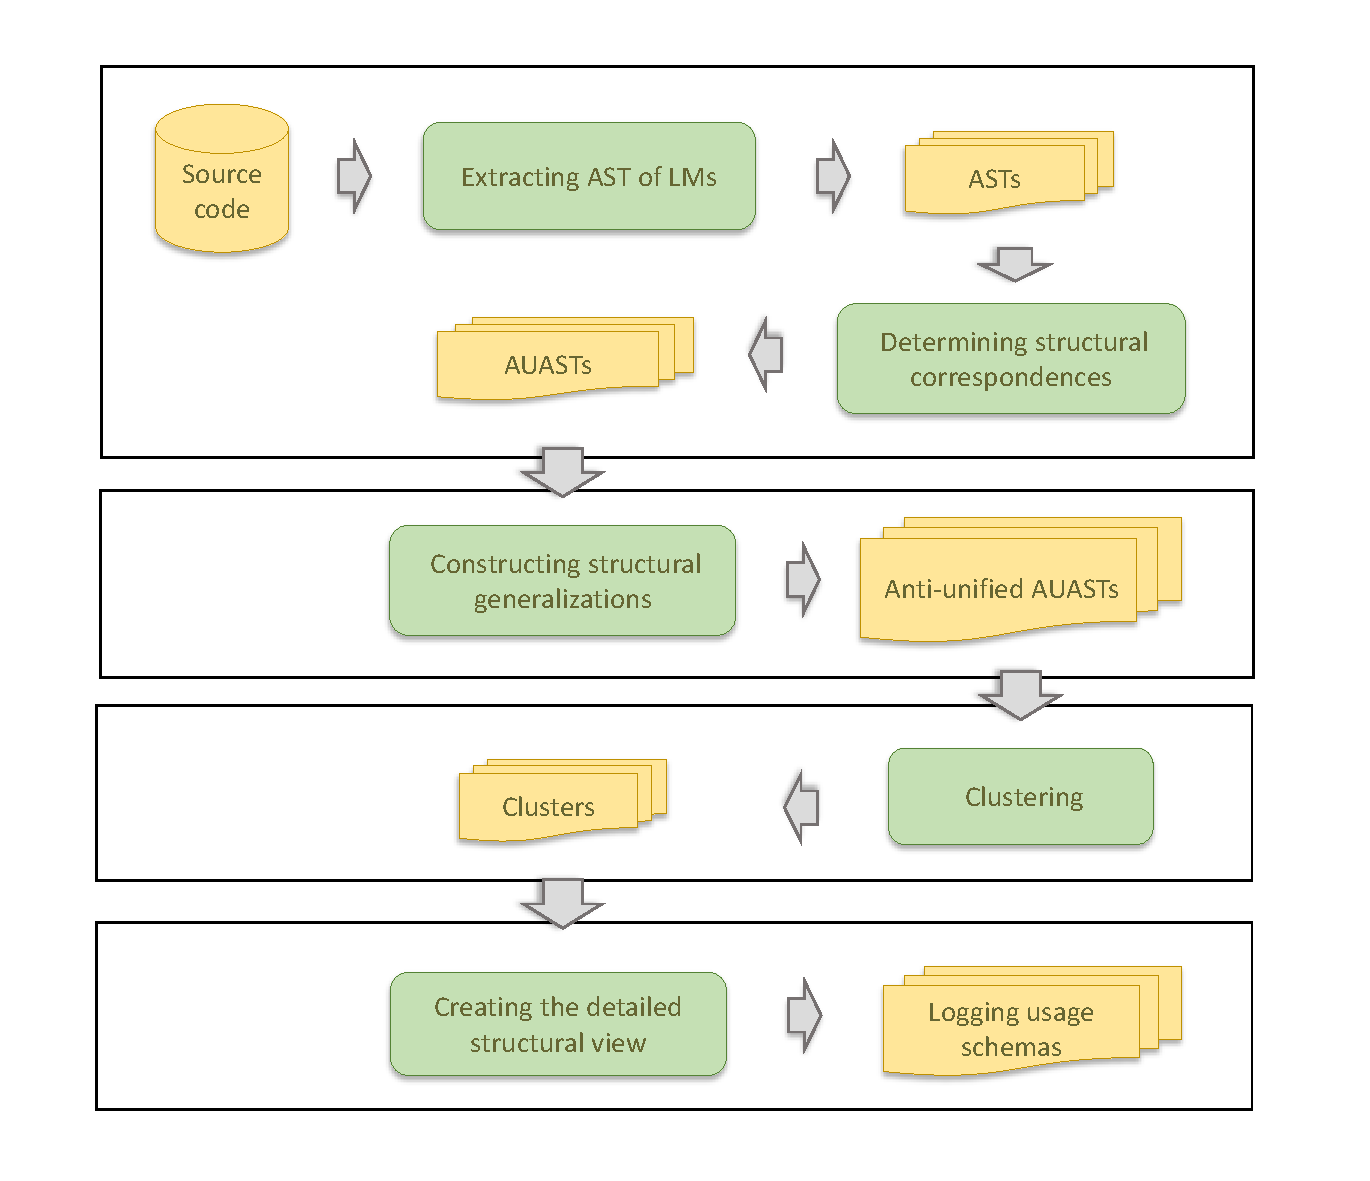
\includegraphics [width = \textwidth]{Drawing4/SystemOverview.pdf}
  \caption{Overview of the approach. %\protect\RW{I don't want to see mention of tools here.  This should be focused on the concepts.}
  }
  \label{fig:system_overview}
\end{figure}

%most similar  or best correspondence?
%constraints wording?
%my emprical study?
%My tool has been applied on the source code of these systems and extracts all logged Java methods from these systems to construct the structural generalizations.
%My evaluation shows ...

\section{Thesis statement} \label{intro-stmt}
%The thesis of this work is that the detailed structural similarities and differences between source code fragments containing log statements can be determined via higher-order anti-unification modulo theories, providing a concise and accurate description of where logging calls do occur in real-world software systems.

The thesis of this work is to characterize where log statements occur in source code by constructing structural generalizations that describe the commonalities and differences between source code fragments containing log statements, thus providing the developers with some guidelines on where to use them effectively in source code. 
%???

\section{Thesis organization} \label{intro-org}
The remainder of the thesis is organized as follows.

Chapter~\ref{ch2} motivates the problem of understanding where to use log statements in source code through a scenario in which a developer attempts to perform a logging task. This scenario outlines the potential problems she may encounter and illustrates that the current logging practice is not sufficiently supported.

Chapter~\ref{background} provides background information that I build atop: abstract syntax trees (ASTs), which are the basic structure I will use for describing software source code; the Eclipse JDT, an industrial framework for producing and manipulating ASTs for source code written in the Java programming language; anti-unification, which is a theoretical approach for constructing structural generalizations; and on Jigsaw, a research tool based on the Eclipse JDT for performing anti-unification.
%clustering added?


Chapters~\ref{background2},~\ref{methodology}, and~\ref{clustering} present the first three steps of my approach. Determining structural correspondences between AUASTs; constructing structural generalizations from an AUAST pair; and classifying a set of AUASTs into separate clusters, respectively. In each chapter, I discuss the implementation of my approach as an Eclipse plug-in, and conduct an experimental study to assess the effectiveness of my approach by applying its tool support on a sample test suite extracted from a real software system.



Chapter~\ref{eval} presents an empirical study I conducted to characterize the location of log statements of four open-source software systems. Chapter~\ref{diss} discusses the results and findings of my work, threats to its validity, and remaining issues. Chapter~\ref{rw} describes work related to my research problem and how it does not adequately address the problem. Chapter~\ref{conc} concludes the dissertation and presents the contributions of this study and future work. %Additional materials appended this dissertation are provided in Appendix A.



